\documentclass{beamer}

\mode<presentation> {

%\usetheme{default}
%\usetheme{AnnArbor}
%\usetheme{Antibes}
%\usetheme{Bergen}
%\usetheme{Berkeley}
%\usetheme{Berlin}
%\usetheme{Boadilla}
%\usetheme{CambridgeUS}
%\usetheme{Copenhagen}
%\usetheme{Darmstadt}
%\usetheme{Dresden}
%\usetheme{Frankfurt}
%\usetheme{Goettingen}
%\usetheme{Hannover}
%\usetheme{Ilmenau}
%\usetheme{JuanLesPins}
%\usetheme{Luebeck}
\usetheme{Madrid}
%\usetheme{Malmoe}
%\usetheme{Marburg}
%\usetheme{Montpellier}
%\usetheme{PaloAlto}
%\usetheme{Pittsburgh}
%\usetheme{Rochester}
%\usetheme{Singapore}
%\usetheme{Szeged}
%\usetheme{Warsaw}


%\usecolortheme{albatross}
%\usecolortheme{beaver}
%\usecolortheme{beetle}
%\usecolortheme{crane}
%\usecolortheme{dolphin}
%\usecolortheme{dove}
%\usecolortheme{fly}
%\usecolortheme{lily}
%\usecolortheme{orchid}
%\usecolortheme{rose}
%\usecolortheme{seagull}
%\usecolortheme{seahorse}
%\usecolortheme{whale}
%\usecolortheme{wolverine}

%\setbeamertemplate{footline} % To remove the footer line in all slides uncomment this line
%\setbeamertemplate{footline}[page number] % To replace the footer line in all slides with a simple slide count uncomment this line

%\setbeamertemplate{navigation symbols}{} % To remove the navigation symbols from the bottom of all slides uncomment this line
}

\usepackage{graphicx} % Allows including images
\usepackage{booktabs} % Allows the use of \toprule, \midrule and \bottomrule in tables
\usepackage{amsfonts}
\usepackage{mathrsfs, bbold}
\usepackage{amsmath,amssymb,graphicx}
\usepackage{mathtools} % gather
\usepackage[export]{adjustbox} % right-aligned graphics

%----------------------------------------------------------------------------------------
%	TITLE PAGE
%----------------------------------------------------------------------------------------

\title["7"]{7: Evaluating, comparing and expanding models}

% \author{Taylor} 
% \institute[UVA] 
% {
% University of Virginia \\
% \medskip
% \textit{} 
% }
\date{10/16/19} 

\begin{document}
%----------------------------------------------------------------------------------------

\begin{frame}
\titlepage 
\end{frame}

%----------------------------------------------------------------------------------------
\begin{frame}
\frametitle{Issues with the introduced criteria}  
\begin{itemize}
\item It is difficult to evaluate the differences of the
  information among all models. The information scales as sample size
  grows.
\item There exists bias in evaluating the predictive performance of
  the selected model. Selection procedure can strongly overfit the data when comparisons are made for a
  large number of models. 
\end{itemize}
\end{frame}


%----------------------------------------------------------------------------------------
\begin{frame}
\frametitle{Bayes Factors}

{\bf Bayes factors} are another way to compare models, two at a time. You compare each model's prior predictive distribution/marginal likelihood/integrated likelihood/evidence:
\begin{block}{Bayes Factors}

\begin{align*}
B_{2,1} &= \frac{p(y \mid H_2)}{p(y \mid H_1)}\\
&= \frac{\int p(y \mid \theta_2, H_2)p(\theta_2 \mid H_2) \text{d}\theta_2}{\int p(y \mid \theta_1, H_1)p(\theta_1 \mid H_1) \text{d}\theta_1}
\end{align*}

assuming $0 < p(y \mid H_i) < \infty$
\end{block}

Models do not have to be nested, and the parameters can be of varying dimension. \\
Unlike frequentist hypothesis testing, it measures the *strength* of one hypothesis over another.

\end{frame}

%----------------------------------------------------------------------------------------
\begin{frame}
\frametitle{Bayes Factors}

$B_{2,1} = \frac{p(y \mid H_2)}{p(y \mid H_1)}$

\begin{center}
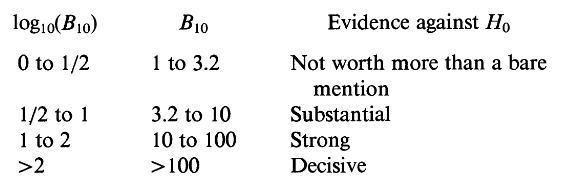
\includegraphics[width=80mm]{bf_scale.png}
\end{center}

From \href{http://www.andrew.cmu.edu/user/kk3n/simplicity/KassRaftery1995.pdf}{http://www.andrew.cmu.edu/user/kk3n/simplicity/KassRaftery1995.pdf}

\end{frame}


%----------------------------------------------------------------------------------------
\begin{frame}
\frametitle{Bayes Factors}

The reason they call it a Bayes factor is because
\[
\text{posterior odds} = \text{Bayes factor} \times \text{prior odds}
\]
\pause

\begin{align*}
\text{posterior odds} &= \frac{p(H_2 \mid y)}{p(H_1 \mid y)} \\
&= \frac{p(y \mid H_2)p(H_2) / p(y)}{p(y \mid H_1)p(H_1) / p(y)} \tag{Bayes rule} \\
&= \frac{p(y \mid H_2)}{p(y \mid H_1)} \frac{p(H_2)}{p(H_1)} \\
&= \text{Bayes factor} \times \text{prior odds}
\end{align*}



\end{frame}


%----------------------------------------------------------------------------------------
\begin{frame}
\frametitle{Bayes Factors}

You should not use improper priors when you calculate Bayes factors because
\[
p(y \mid H_1) = \int p(y \mid \theta_1, H_1)p(\theta_1 \mid H_1) \text{d}\theta_1
\]
is not a density (homework question), and the normalizing constant will be ambiguous.

\end{frame}

%----------------------------------------------------------------------------------------
\begin{frame}
\frametitle{Bayes Factors}

Even noninformative proper priors can be ``biased" towards one of the hypotheses. 
\newline

% Consider HW question on page 194. 
% \newline

Consider the following example of the {\bf Jeffreys-Lindley's paradox}:
\begin{enumerate}
\item under $H_1$: $\theta = 0$ with prior probability $1$
\item $p(\bar{y} \mid H_1)  = (2\pi)^{-1/2}n^{1/2} \exp\left[-\frac{n}{2}\bar{y}^2 \right]$
\item $p(\theta \mid H_2 ) = N(0,\tau^2)$
\item $p(\bar{y} \mid H_2) = \int p(\bar{y} \mid \theta, H_2)p(\theta \mid H_2)\text{d}\theta = [2\pi(\tau^2 + n^{-1})]^{-1/2} \exp\left[-\frac{1}{2(\tau^2 + n^{-1})}\bar{y}^2 \right]$
\end{enumerate}
so
\[
B_{1,2} = (n\tau^2 + 1)^{1/2} \exp\left[-\frac{\bar{y}^2}{2}\left(n - \frac{1}{(\tau^2 + n^{-1})}\right) \right]
\]

\end{frame}

%----------------------------------------------------------------------------------------
\begin{frame}[fragile]
\frametitle{Bayes Factors: The Jeffreys-Lindley's paradox}

Say $\bar{y} = 1.5$ and $n = 10$. Then our p-value for the null is $2.101436e-06$, but 
\begin{center}
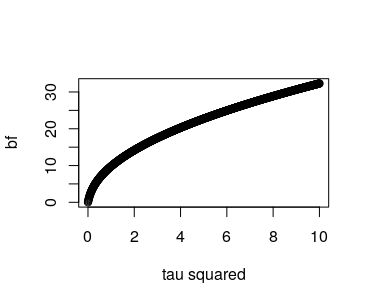
\includegraphics[width=75mm]{jf_paradox.png}
\end{center}

Different decisions based on whether we are frequentist or Bayesian?!

% \begin{verbatim}
% n <- 10
% ybar <- 1.5
% freq_test_stat <- sqrt(n)*ybar
% 2*pnorm(-abs(freq_test_stat))
% bf <- function(tausq) { 
%   (n*tausq + 1)^(1/2)*exp( -(ybar^2/2 ))*( n - 1 / (tausq + 1/n) ) 
% }
% tausq_grid <- seq(0,10, .01)
% plot(tausq_grid, bf(tausq_grid), xlab = "tau squared", ylab = "bf")
% \end{verbatim}



\end{frame}

%----------------------------------------------------------------------------------------
\begin{frame}
\frametitle{Bayes Factors}

If you can't derive $p(y \mid H_i)$, then it must be approximated. Noticing that the joint $p(y \mid \theta_i, H_i)p(\theta_i \mid H_i)$ is an unnormalized target, here is the justification behind importance sampling:

\begin{align*}
p(y \mid H_i) &= \int p(y \mid \theta_i, H_i)p(\theta_i \mid H_i) \text{d}\theta_i \\
&= \int \frac{p(y \mid \theta_i, H_i)p(\theta_i \mid H_i)}{q(\theta_i)}q(\theta_i) \text{d}\theta_i \\
&\leftarrow \frac{1}{S}\sum_{s=1}^S \frac{p(y \mid \theta^s_i, H_i)p(\theta^s_i \mid H_i)}{q(\theta^s_i)}
\end{align*}

where $\theta^s_i \sim q(\theta_i)$.
\newline

% Importance sampling will be discussed further in chapter 10.
\end{frame}

% %----------------------------------------------------------------------------------------
% \begin{frame}
% \frametitle{Bayes Factors and the ``Worst Monte Carlo Method Ever" }

% One might tempted to use the posterior samples, too:

% \begin{align*}
% p(y \mid H_i)
% &= \left[  \int \frac{p(y \mid \theta_i,  H_i)p(\theta_i \mid H_i)}{p(y \mid H_i) p(y \mid \theta_i, H_i) } \text{d}\theta_i \right]^{-1}\\
% &= \left[  \int \frac{p(\theta_i\mid y,  H_i) }{p(y \mid \theta_i, H_i) } \text{d}\theta_i \right]^{-1} \tag{Bayes' theorem}\\
% & \leftarrow  \left[  \frac{1}{S}\sum_{s=1}^S\frac{1 }{p(y \mid \theta_i^s, H_i) } \right]^{-1}
% \end{align*}

% where $\theta^s_i \sim p(\theta_i\mid y,  H_i)$ are samples from the posterior. 
% \newline

% However, this estimator often has infinite variance. There are a number of adjustments to this approach. 
% \end{frame}

%----------------------------------------------------------------------------------------
\begin{frame}
\frametitle{Bayes Factors}

Under certain conditions, the {\bf Bayesian Information Criterion} or {\bf Schwarz Information Criterion} approximates the log of integrated likelihood. 
\[
BIC(H_i) = \log p(y \mid \hat{\theta}, H_i) - k \log(n)
\]
where $n$ is the number of data points, and $k$ is the dimension of $\theta$.
\newline

You don't even need to specify a prior. However, BIC requires the knowledge of number of parameters, which can be a hard to obtain in complicated models.

\end{frame}


\end{document} 



%%% Local Variables:
%%% mode: latex
%%% TeX-master: t
%%% End:
